\section{Versuchsaufbau und Versuchdurchführung}

\subsection{Messung bis 1 bar }

\begin{flushleft}
    Der Versuch wird wie in Abbildung \ref{Abbildung3} aufgebaut.
    Nach dem Aufbau wird zuerst der Druck der Umgebungsluft gemessen und notiert.
    Danach wird der Mehrhalskolben evakuiert, indem der Absperrhahn sowie das Drosselventil geöffnet und das Belüftungsventil geschlossen werden.
    Als nächstes wird die Wasserstrahlpumpe angemacht und laufen gelassen, bis das Manometer einen konstanten Druck anzeigt.
    Wenn ein konstanter Druck herrscht, wird erst das Drosselventil, dann der Absperrhahn und als letztes die Wasserstrahlpumpe geschlossen und die Wasserkühlung wird angestellt, damit der Dampf wieder kondensiert.
    Die Heizhaube wird angestellt und je später es im Erhitzungsvorgang wird umso mehr wird die Wasserkühlung verringert.
    Nun werden insgesamt 50 Wertepaare, zusammensetzend aus Temperatur und Druck, aufgenommen in einem gleichbleibenden Abstand.
    Beendet wird die Messung wenn das Manometer 1 bar anzeigt, also Umgebungsdruck.
\end{flushleft}

\begin{figure}[H]       
    \centering
    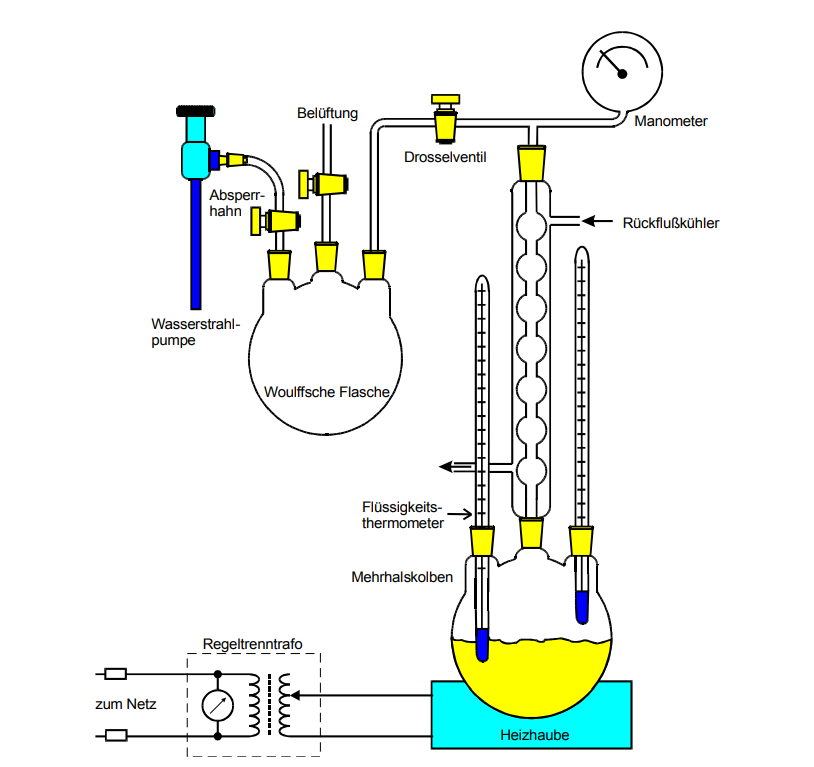
\includegraphics[height=120mm]{bilder/A1.png}
    \caption{der Aufbau des ersten Versuchs \cite{a1}.\label{Abbildung3} }
\end{figure}

\subsection{Messung von 1 bis 15 bar}

\begin{flushleft}
    In dem nächsten Versuchsteil wird die Apparatur gewechselt und der Aufbau sieht aus wie in Abbildung \ref{Abbildung4}.
    Hierbei wird vor Beginn der Stahlbolzen komplett mit destilliertem und entgastem Wasser gefüllt.
    Anschließend wird die Heizwicklung aktiviert und es werden wieder Datenpaare wie in dem ersten Versuch aufgenommen.
    Diesmal sind es wieder Druck und Temperatur, jedoch werden diese Werte bei jedem halben bar anstieg notiert. 
\end{flushleft}

\begin{figure}[H]       
    \centering
    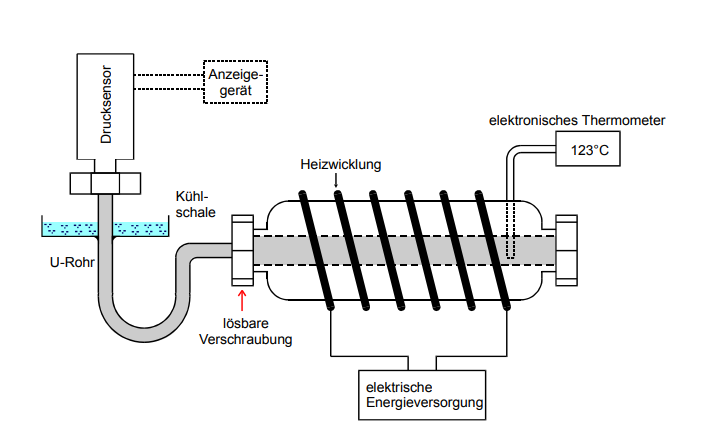
\includegraphics[height=75mm]{bilder/A2.png}
    \caption{Der Aufbau des zweiten Versuchs \cite{a1}. \label{Abbildung4} }
\end{figure}